\chapter{Infrastructure}\label{ch:infrastructure}
This chapter serves as a way to introduce the tools that have been employed during the development of this project. All of them are \emph{open-source}. The transparency provided by the open-source platforms is a major advantage, because the third-party software can be easily integrated in our specific applications, which are mainly written in \emph{Python}\footnote{\url{https://www.python.org/}}. These applications will reach a high-quality performance faster than if they would have been written from scratch.

\section{Keras framework}\label{sec:keras}
As stated by \emph{Keras} documentation~\cite{chollet2015keras}: ``Keras is a high-level \emph{neural network library}, written in Python and capable of running on top of either TensorFlow or Theano". TensorFlow and Theano are open-source libraries for numerical computation, optimized for GPU and CPU. Keras treats them as its \textit{backends}. The main version used in this project is Keras 1.2.2, although it has been recently updated to 2.0.4 version because of its backward compatibility. In this work, Keras has run on top of \emph{Theano}\footnote{\url{http://deeplearning.net/software/theano/index.html}}, optimized for CPU and has been employed to train and implement several \glspl{cnn}.

In the following sections, the main elements that make up a neural network built with Keras are analyzed, starting with the \emph{\textit{model} object}, its core component.

\subsection{Models}\label{subsec:models}
Every neural network in Keras is defined as a \emph{\textit{model}}. For those models which can be built as a stack of \textit{layers} (see Section~\ref{subsec:layers}), Keras provides the \emph{\textit{.Sequential()} object}. In the following chapter, an example of a sequential model built with Keras is shown in Figure~\ref{fig:model}. It is also possible to build more complex models with multiple outputs and shared layers using the \emph{Keras functional API}.

Sequential models have several methods, and the following ones are essential for the learning process:
\begin{description}
	\item[\textit{.compile()}] It configures the \emph{learning process}. Its main arguments are:
	\begin{itemize}
		\item \textbf{\textit{loss}}: name of the \emph{cost function} that measures the difference between predicted and real labels. In this project, the \emph{categorical cross-entropy}, also known as log loss, has been used. This function returns the cross-entropy between an approximating distribution $q$ and a true distribution $p$~\cite{theano} and it's defined as:
		\begin{equation}\label{eq:categorical_crossentropy}
		H(p,q)=-\Sigma_{x}p(x)\log(q(x))
		\end{equation}		
		Other loss functions, such as mean squared error (MSE) and mean absolute error, are also provided by Keras.
		
		\item \textbf{\textit{optimizer}}: name of the optimizer that will update the weights values during training in order to minimize the loss function. The chosen algorithm for this task is \emph{ADADELTA}. This optimizer is an extension of the \emph{gradient descent} optimization method, and has the particularity of adapting automatically the learning rate during training~\cite{DBLP:journals/corr/abs-1212-5701}.				
		Other optimization methods, such as Adagrad, Adamax and Adam, are also available.
		
		\item \textbf{\textit{metrics}}: name of the functions that must be computed during training and testing for performance evaluation. \emph{Accuracy} is the only function which will be evaluated with Keras through this project, besides the loss function, which is automatically computed. It is defined as the proportion of examples for which the model produces the correct output~\cite{Goodfellow-et-al-2016}.			
		Other measurements about the performance of the model are obtained with the \emph{Scikit-learn} library (see Section~\ref{sec:skoctave}).
	\end{itemize}
\end{description}

\begin{description}
	\item[\textit{.fit()}] It trains the model. The following arguments are required:
	\begin{itemize}
		\item \textbf{\textit{x}, \textit{y}}: training samples and labels. They must be defined as \emph{Numpy arrays}\footnote{\url{http://www.numpy.org/}}.
		
		\item \textbf{\textit{batch\_size}}: number of samples that are evaluated before updating the weights. It defaults to 32.
		
		\item \textbf{\textit{epochs}}: number of iterations over the whole dataset that are going to be executed. It defaults to 10.
		
		\item \textbf{\textit{callbacks}}: list of callbacks (see Section~\ref{subsec:callbacks}) that are going to be applied during training. It defaults to \textit{None}.
		
		\item \textbf{\textit{validation\_split} or \textit{validation\_data}}: in Keras, there are two alternatives to provide a validation dataset. On the one hand, it is possible to pass the validation data as a Numpy array to the \textit{validation\_data} argument. On the other hand, a fraction of the training samples can be set as validation data through the \textit{validation\_split} argument. \textit{validation\_data} and  \textit{validation\_split} arguments are mutually exclusive, so just one of them can be used.
		
		\item \textbf{\textit{shuffle}}: a boolean that determines whether to shuffle training data or not. If data are not shuffled during training, samples belonging to the same class can be presented consecutively. In that case, the model will be forced to learn the features of a certain class. When the model starts to see samples of the next class, it fits to the new data and forgets the previously learned feature. If data are sorted by classes, this process goes on and on leading to a worse performance.
	\end{itemize}
\end{description}

\begin{description}
	\item[\textit{.predict()}] It takes a sample and returns the label predicted by the model.
\end{description}

\begin{description}
	\item[\textit{.evaluate()}] It takes a set of samples and labels and evaluates the \emph{model performance}, returning a list of the \textit{metrics} previously defined.
\end{description}

\begin{description}
	\item[\textit{.save()}] It stores the model into a \emph{\gls{hdf5} file} (see Section~\ref{sec:hdf}), which will contain the weights, architecture and training configuration of the model.
\end{description}

\begin{description}
	\item[\textit{.load\_model()}] It loads a model from a \emph{\gls{hdf5} file}.
\end{description}

\subsection{Layers}\label{subsec:layers}
As it has been said before, the models are usually built as a \emph{stack of layers}. These layers are added to the model using the \textit{.add()} method, inside of which the kind of layer is declared and its particular parameters are set. Several kinds of layers are available, but only the ones that have been used in this project are going to be described.
\begin{description}
	\item[Convolutional layer.] This particular layer is the one that turns the neural network into a \emph{\gls{cnn}}. It is formed by a certain amount of \emph{filters/kernels} with a fixed size. These filters are convolved with the input volume, generating each one a \emph{feature or activation map} which will tell us to what extent the feature learned by that particular filter is present in that volume~\cite{cs231n}. In our case, the input volume will be a three dimensional matrix defined by its width (number of columns), height (number of rows) and depth (number of channels). It's important to note that the number of channels of the filter will be equal to the number of channels of the input, which implies that each filter will generate just one activation map, instead of generating one for each channel. 
	
	Keras provides different kinds of convolutional layers depending on the input dimensions: \textit{Conv1D}, \textit{Conv2D} and \textit{Conv3D}. These are the main arguments required by Keras to define a convolutional layer:
	\begin{itemize}
		\item \textbf{\textit{filters}}: number of filters.
		
		\item \textbf{\textit{kernel\_size}}: width and height of the filters.
		
		\item \textbf{\textit{strides}}: how many pixels the filter must be shifted before applying the next convolution. It defaults to 1.
		
		\item \textbf{\textit{padding}}: it can be \textit{valid} or \textit{same}. If \textit{valid} mode is set, no padding is applied, resulting in an output that will be smaller than the input. However, if \textit{same} mode is set, the input will be padded with zeros in order to produce an output that preserves the input size. It defaults to \textit{valid}.
	\end{itemize}

	Figure~\ref{fig:convlayer} shows a detailed representation of the operation performed by convolutional layers. In Figure~\ref{fig:convlayer}(a), the filter $w_0$ (3x3x3) is convolved with the input volume (5x5x3). In this example, as padding is set to~1~and stride is equal~2, the operation will return a~3x3~activation map. The same procedure is followed in Figure~\ref{fig:convlayer}(b) with the filter $w_1$. It generates another~3x3~activation map, ending up with a~3x3x2~output. To clarify this process, let's see how to obtain the first element in the second row of the activation map returned by the filter $w_0$, i.e. the element within the green square in Figure~\ref{fig:convlayer}(a).
	\begin{enumerate}
		\item An element-wise or \emph{Hadamard product} is performed between the filter $w_0$ and the corresponding region (\emph{receptive field}) of the input volume $x$.
		\begin{equation}
		z_1=x[:,:,0]_{r. field}\odot{w_0[:,:,0]} = 
		\begin{bmatrix}
		0\cdot 1 & 1\cdot 0 & 1\cdot 0\\
		0\cdot 1 & 1\cdot 1 & 2\cdot -1\\
		0\cdot -1 & 2\cdot -1 & 0\cdot -1
		\end{bmatrix}=
		\begin{bmatrix}
		0 & 0 & 0\\
		0 & 1 & -2\\
		0 & -2 & 0
		\end{bmatrix}
		\end{equation}
		\begin{equation}
		z_2=x[:,:,1]_{r. field}\odot{w_0[:,:,1]} = 
		\begin{bmatrix}
		0\cdot -1 & 2\cdot -1 & 2\cdot -1\\
		0\cdot 0 & 1\cdot -1 & 2\cdot 0\\
		0\cdot 1 & 0\cdot 1 & 2\cdot 0
		\end{bmatrix}=
		\begin{bmatrix}
		0 & -2 & -2\\
		0 & -1 & 0\\
		0 & 0 & 0
		\end{bmatrix}
		\end{equation}
		\begin{equation}
		z_3=x[:,:,2]_{r. field}\odot{w_0[:,:,2]} = 
		\begin{bmatrix}
		0\cdot 0 & -1\cdot 2 & 1\cdot 0\\
		0\cdot 0 & -1\cdot 0 & 1\cdot 1\\
		0\cdot 0 & 0\cdot 0 & -1\cdot 0
		\end{bmatrix}=
		\begin{bmatrix}
		0 & -2 & 0\\
		0 & 0 & 1\\
		0 & 0 & 0
		\end{bmatrix}
		\end{equation}		
		\item Then, all elements of the three resulting matrices are added together.
		\begin{equation}
		\Sigma z_1 + \Sigma z_2 + \Sigma z_3 = -3 - 5 -1 = -9
		\end{equation}
		\item Finally, the \emph{bias} ($b_0$) is added to the scalar returned by the previous addition. Bias allows to \emph{shift} the input of the activation function away from the origin, like the constant in a linear function. For instance, if the receptive field is filled with zeros, the bias gives the opportunity of generating a non-zero output. Activation functions will be discussed later in this section.
		\begin{equation}
		o[:,:,0] = -9 + b_0 = -8
		\end{equation}
		\item To compute the value of the next element of the activation map, the same operation is applied to the next receptive field which, according to the stride that has been set, must be~2~pixels away from the previous one.
	\end{enumerate} 
	
	\begin{figure}
		\centering
		\begin{subfigure}{0.7\textwidth}
			\centering
			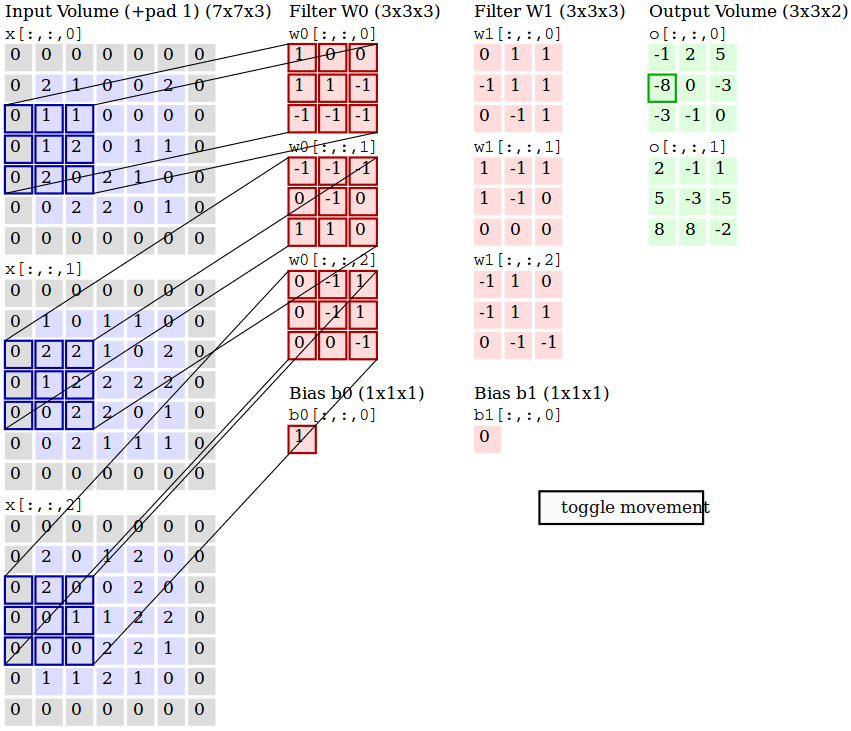
\includegraphics[width=1\linewidth]{figures/convlayer_anime1big.png}
			\caption{}
		\end{subfigure}
		\begin{subfigure}{0.7\textwidth}
			\centering
			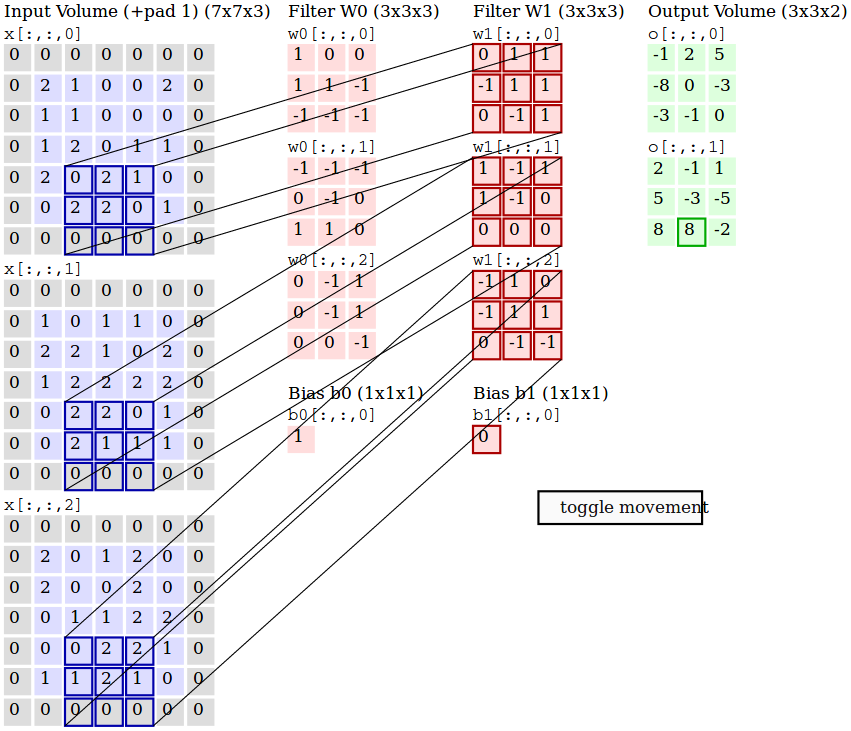
\includegraphics[width=1\linewidth]{figures/convlayer_anime2big.png}
			\caption{}
		\end{subfigure}
		\caption{Example of operation of a convolutional layer (source~\cite{cs231n}): (a) filter $w_0$; (b) filter $w_1$.}
		\label{fig:convlayer}
	\end{figure}
	
	A more intuitive and general representation of how a convolutional layer works is shown in Figure~\ref{fig:convlayersimple}.
	\begin{figure}
		\centering
		\includegraphics[width=0.9\linewidth, keepaspectratio]{figures/cnn.png}
		\caption{Intuitive representation of a convolutional layer.}
		\label{fig:convlayersimple}
	\end{figure}	
\end{description}

\begin{description}
	\item[Pooling layer.] It shifts a window of a certain size along the input volume applying an operation (mean or maximum) that will return a \emph{\textit{downsampled} version} of it, reducing the computational cost and avoiding overfitting~\cite{Scherer2010Evaluation}. Figure~\ref{fig:pooling} shows how the pooling operation is applied.

	\begin{figure}
		\centering
		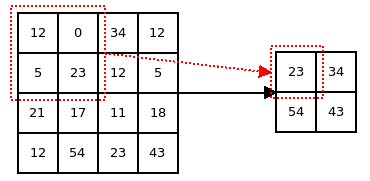
\includegraphics[width=10cm, keepaspectratio]{figures/pooling.png}
		\caption{Example of a max. pooling operation.}
		\label{fig:pooling}
	\end{figure}
	
	Depending on the dimensions of the input and the operation applied, Keras provides several pooling layers: \textit{MaxPooling1D}, \textit{MaxPooling2D}, \textit{MaxPooling3D}, \textit{AveragePooling1D}... The main arguments required by Keras to define these layers are:
	\begin{itemize}
		\item \textbf{\textit{pool\_size}}: size of the window that is shifted along the input.
		\item \textbf{\textit{strides}}: how many pixels the window must be shifted before applying the next operation.
	\end{itemize}
\end{description}

\begin{description}
	\item[Dense layer.] Fully-connected layers in Keras are defined as \textit{Dense layers}. In a \emph{fully-connected layer}, every neuron is connected to every activation (i.e. output) of the previous one~\cite{cs231n}. The main argument of this layer is:
	\begin{itemize}
		\item \textbf{\textit{units}}: number of neurons.
	\end{itemize}
	Figure~\ref{fig:fc} shows the diagram of a dense layer. The weights of each connection are represented by the thickness of the lines.
	\begin{figure}
		\centering
		\includegraphics[width=0.4\linewidth, keepaspectratio]{figures/FCLayer.png}
		\caption{Diagram of a dense or fully-connected layer (source~\cite{fc}).}
		\label{fig:fc}
	\end{figure}
\end{description}

\begin{description}
	\item[Activation layers.] In Keras models, an activation function can be declared as a layer itself or as an argument within the \textit{.add()} method of the previous layer. Keras provides several \emph{activation functions}, such as sigmoid, linear, \gls{relu} and softmax. These are the ones that have been used during the development of this project:
	\begin{itemize}
		\item \textbf{\gls{relu}}: this activation function introduces a \emph{non-linearity} right after each convolutional layer, allowing the \gls{cnn} to learn more complex features. It's defined as:
		\begin{equation}\label{eq:relu}
		g(z)=\max(0,z)
		\end{equation}
		Figure~\ref{fig:activations} shows \gls{relu} function plotted in the interval~$[-1,1]$.
		\begin{figure}
			\centering
			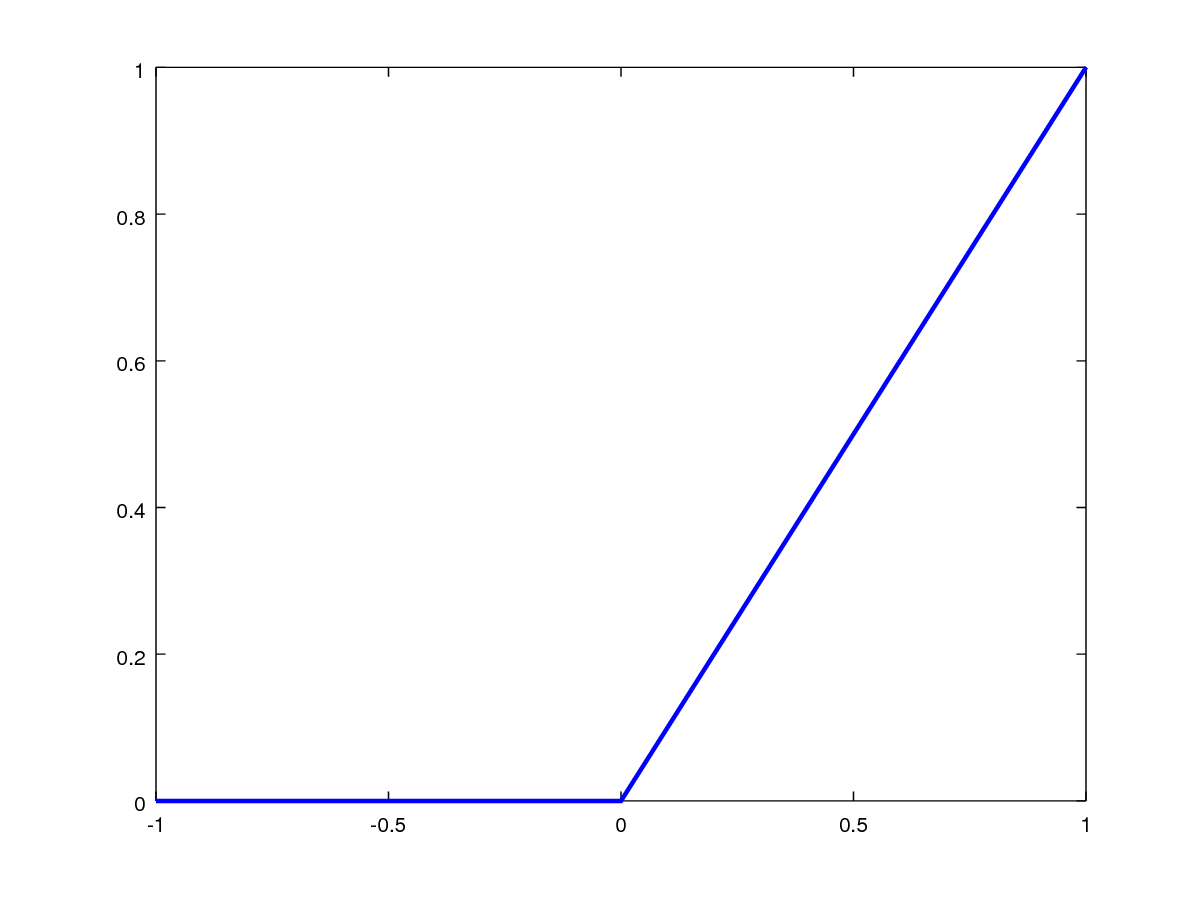
\includegraphics[width=0.6\linewidth]{figures/relu.png}
			\caption{\gls{relu} activation function.}
			\label{fig:activations}
		\end{figure}
		
		\item \textbf{Softmax}: this activation function is very useful when is placed after the \emph{output layer} of classification tasks. It takes a vector of real values $z$ and returns a new vector of real values in the range [0,1]. The $N$ elements of the output vector can be considered \emph{probabilities} because the softmax function ensures that they sum up to 1. It is defined as follows:
		\begin{equation}\label{eq:SoftMax}
		\mathrm{softmax}(z)_i=\frac{\exp(z_i)}{\Sigma_{j}{\exp(z_j)}} \quad \mathrm{for} \ j=1, ...,N
		\end{equation}
	\end{itemize}
	These equations and definitions have been extracted from~\cite{Goodfellow-et-al-2016}. 
	
\end{description}

\begin{description}
	\item[Flatten layer.] It \textit{flattens} the input. For instance, it converts the activation maps returned by the convolutional layers into a \emph{vector of weights} before being connected to a dense layer. It takes no arguments.
\end{description}

\begin{description}
	\item[Dropout layer.] It's considered a \emph{regularization layer}, because its main purpose is to avoid overfitting. Dropout is a technique that randomly \emph{\textit{switches-off}} a fraction of hidden units during training~\cite{srivastava2014dropout}. It can also be understood as a technique that ``trains an ensemble consisting of all subnetworks that can be structured by removing non-output units from an underlying base network"~\cite{Goodfellow-et-al-2016}, as it can be seen in Figure~\ref{fig:dropout}.

	\begin{figure}
		\centering
		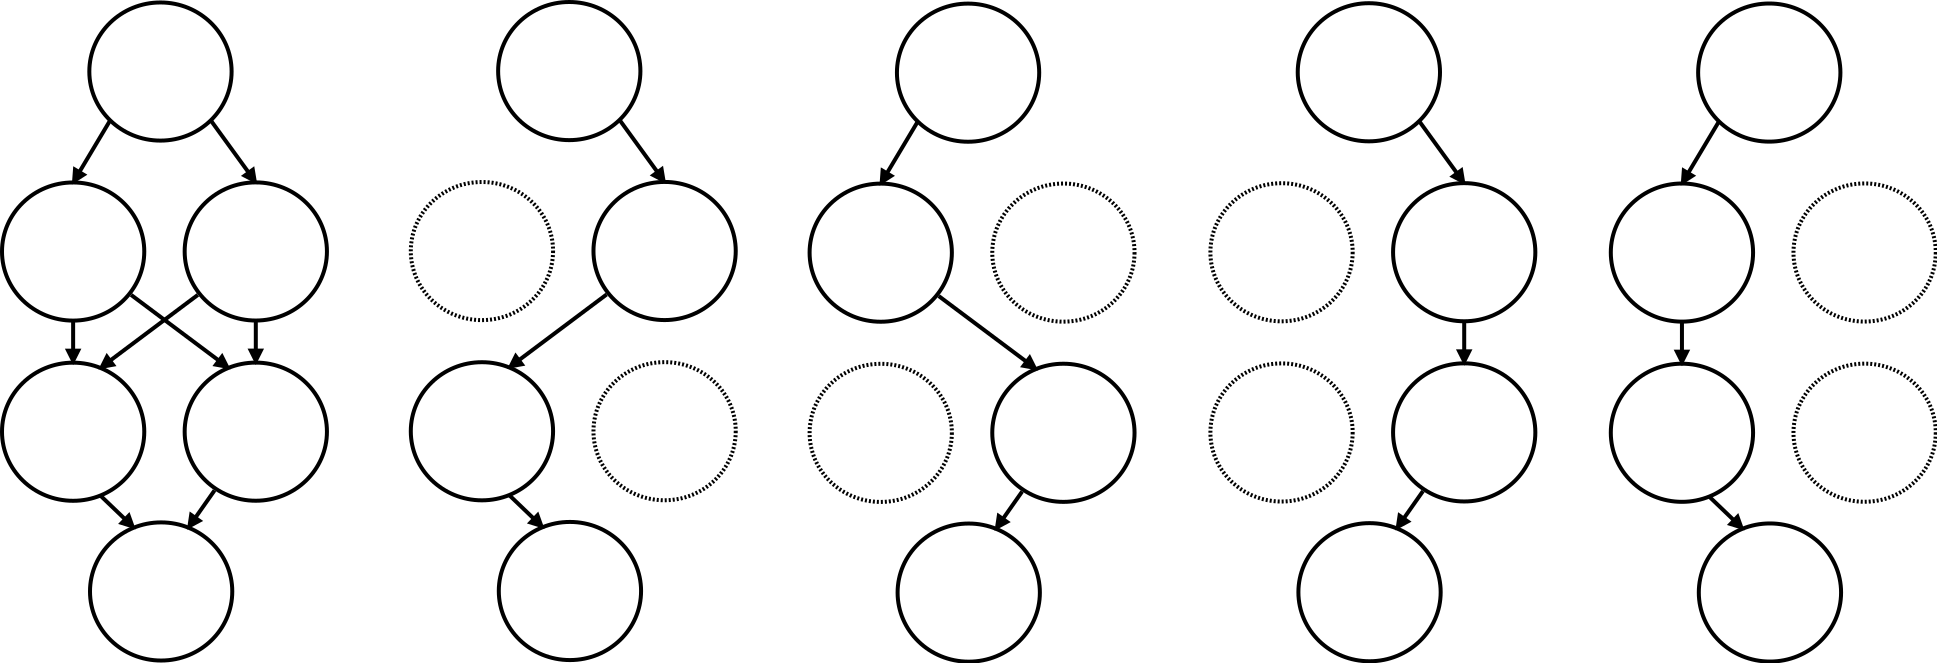
\includegraphics[width=1\linewidth, keepaspectratio]{figures/dropout.png}
		\caption{Subnetworks generated when using dropout.}
		\label{fig:dropout}
	\end{figure}	

	 This layer, as other regularization layers (i.e. GaussianNoise layer), is only active during training. It's main argument is:
	\begin{itemize}
		\item \textbf{\textit{rate}}: fraction of units that must be dropped.
	\end{itemize}
	
\end{description}

\subsection{Callbacks} \label{subsec:callbacks}
As defined by Keras documentation~\cite{chollet2015keras}, \emph{callbacks} are a set of functions applied at given stages while the model is being trained. They can be used to take a look at the state of the model during training. The built-in callbacks that have been used for this project are:
\begin{itemize}
	\item \textbf{\textit{.History()}}: it is automatically applied to every Keras model and is returned by the \textit{.fit()} method. After each epoch, this callback evaluates the declared \textit{metrics} with the validation dataset and saves the results.
	
	\item \textbf{\textit{.EarlyStopping()}}: it monitors the value of a given function and forces the model to stop training when that function has stopped improving. It has a \emph{\textit{patience}} argument, which determines how many epochs in a row without improving must be tolerated before the model stops training. Setting up an appropriate \emph{stopping criteria} may prevent the model from overfitting.
	
	\item \textbf{\textit{.ModelCheckpoint()}}: it saves the model and its weights after each epoch. It can be configured to overwrite the model only if a certain \textit{metric} has improved with respect to the previous best result, saving the best \textit{version} of it.
\end{itemize}

Additionally, Keras provides the \textit{Callback} base class that can be used to build \emph{user-defined callbacks}.

\subsection{Image preprocessing}\label{subsec:utils}
\emph{Image preprocessing} is a key factor in every computer vision application. Specifically, in \gls{ml}, besides adapting images and emphasizing certain particularities before training that can improve the model performance (i.e. edge detection), it can be used to avoid \emph{overfitting} through data augmentation. \emph{Data augmentation}~\cite{DBLP:journals/corr/WongGSM16} consists in taking the original images of the dataset and applying transformations to them. This operation adds more variability to samples, leading to a better generalization.

This functionality is included in Keras thanks to the \emph{\textit{.ImageDataGenerator()} method}. It returns a batch generator which randomly applies the desired transformations to random samples of the dataset provided by the user. Built-in transformations like rotation, shifting and zooming, are passed as arguments to the aforementioned method. Additionally, it's possible to build a user-defined function and pass it as an argument as well. The dataset and the batch size are defined through the \emph{\textit{.flow()} method}. During training, the generator will loop until the number of samples per epoch and the number of epochs set by the user are satisfied.

\subsection{Utils}
Keras includes a module for multiple supplementary tasks called \emph{\textit{Utils}}. The most important functionality for the project provided by this module is the \emph{\textit{.HDF5Matrix()} method}. It reads the \emph{\gls{hdf5} datasets} (see Section~\ref{sec:hdf}), which are going to be used as inputs to the neural networks.

\section{HDF5 file format}\label{sec:hdf}
During the development of this project, large amounts of data have been processed. Because of that, an efficient way of reading and saving these data have been an important point. Keras employs the \emph{\gls{hdf5} file format} to save models and read datasets.

According to \gls{hdf5} documentation~\cite{hdf5}, it is a \emph{hierarchical data format} designed for high volumes of data with complex relationships. While relational databases employ tables to store data (e.g. SQL), \gls{hdf5} supports \emph{n-dimensional datasets} and each element in the dataset may be as complex as needed.

In order to deal with \gls{hdf5} files, the \emph{h5py}\footnote{\url{http://www.h5py.org/}} library for Python has been employed.

\section{Scikit-learn and Octave}\label{sec:skoctave}
\emph{Scikit-learn} is a \gls{ml} library that includes a wide variety of algorithms for clustering, regression and classification~\cite{scikit-learn}. It can be used at every stage of the \gls{ml} workflow: preprocessing, training, model selection and evaluation.

Scikit-learn functions have been used to evaluate the neural networks developed with Keras. Using a tool that is \emph{independent from Keras} enables the comparison of the results achieved by different neural network libraries (e.g. Keras and Caffe). These are the evaluation parameters which have been employed in this project (equations and definitions obtained from~\cite{scikit-doc}):
\begin{itemize}
	\item \textbf{Precision}: ability of the classifier not to label as positive a sample that is negative.
	\begin{equation}\label{eq:precision}
	\textrm{precision}=\frac{true_{positives}}{true_{positives}+false_{positives}}
	\end{equation}
	
	\item \textbf{Recall}: ability of the classifier to find all the positive samples.
	\begin{equation}\label{eq:recall}
	\textrm{recall}=\frac{true_{positives}}{true_{positives}+false_{negatives}}
	\end{equation}
	
	\item \textbf{Confusion matrix}: a two dimensional matrix where the element in the position $i,j$ represents the number of samples that belongs to the group $i$ but have been classified as belonging to group $j$. True predictions can be found in the diagonal of the matrix, where $i=j$. An example of a confusion matrix computed with Scikit-learn can be found in Figure~\ref{fig:conf_mat}.
\end{itemize}

Besides the functions that have just been mentioned, \emph{accuracy} and \emph{log loss} have also been used and they're defined as in Section~\ref{subsec:models}.

\emph{GNU Octave}~\cite{octave} is a scientific programming language compatible with \emph{Matlab}. It provides powerful tools for plotting. In this work, it has been used to visualize the aforementioned parameters collected with Scikit-learn about the performance of the models.

\begin{figure}
	\centering
	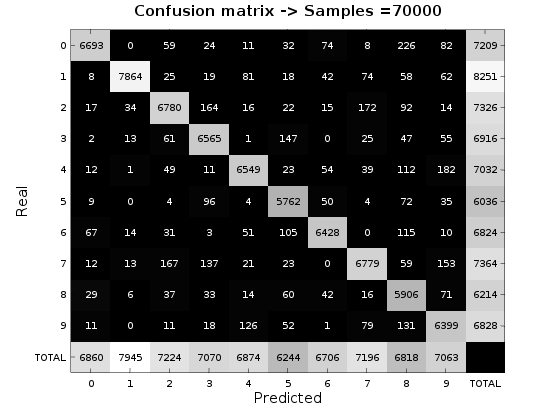
\includegraphics[width=0.8\linewidth, keepaspectratio]{figures/conf_mat.png}
	\caption{Example of a confusion matrix.}
	\label{fig:conf_mat}
\end{figure}

\section{JdeRobot framework}\label{sec:jderobot}
\emph{JdeRobot} is an open source middleware for robotics and computer vision~\cite{jderobot}. It has been designed to simplify the software development within these fields. It is mostly written in C\nolinebreak[4]\hspace{-.05em}\raisebox{.4ex}{\tiny\bf ++} language and is structured like a collection of components (tools and drivers) that communicate to each other through \emph{ICE interfaces}\footnote{\url{https://zeroc.com/products/ice}}. It is also compatible with the robotics middleware \emph{ROS}\footnote{\url{http://www.ros.org/}}, which allows the interoperation of ROS nodes and JdeRobot components. This flexibility makes it very useful for our application. The version employed in this work is JdeRobot 5.5. This middleware and, more specifically, its \emph{\textit{cameraserver} driver}, is going to be employed to capture images from different video sources that will feed the digit classifier component.

\subsection* {\textit{cameraserver}}
According to JdeRobot documentation~\cite{jderobot}, this driver can serve images both from real cameras and from video files. It communicates with other components thanks to the \emph{ICE \textit{Camera} interface}.

In order to use \textit{cameraserver}, its \emph{configuration file} has to be properly set. These are the parameters that must be specified:
\begin{itemize}
	\item The \emph{network address} where the server is going to be listening.
	
	\item Parameters related with the \emph{video stream}: URI, frame rate, image size and format.
\end{itemize}

\section{DroidCam}\label{sec:droidcam}
On the one hand, \emph{DroidCam} is an application for Android which serves the images captured with a \emph{smartphone camera}~\cite{droidcam}. On the other hand, it is a client for Linux which receives the video stream served by Android and makes it accessible for the computer as a \emph{v4l2\footnote{\url{https://www.linuxtv.org/wiki/index.php/Main_Page}} device driver}. The Linux client can be connected to the phone camera over a USB cable or a WiFi network and allows the user to control camera flash, auto-focus and zoom. DroidCam provides the address at which the Linux client must be listening to receive the images. Besides that, it provides a URL that can be used to access the video stream from any browser. The DroidCam version used in this work is DroidCam 6.4.8. It will enlarge the list of possible video sources for the digit classifier component by serving the images of a smartphone camera.

An example of usage can be seen in Figure~\ref{fig:droidcam}. First, the Android app is opened. It shows the address where the video will be served (see Figure~\ref{fig:droidcam}(a)). Then, the address is set in the Linux client (see Figure~\ref{fig:droidcam}(b)). Finally, when the \textit{Connect} button is pressed, the connection is established (see Figure~\ref{fig:droidcam}(c)).
\begin{figure}
	\centering
	\begin{subfigure}{0.33\textwidth}
		\centering
		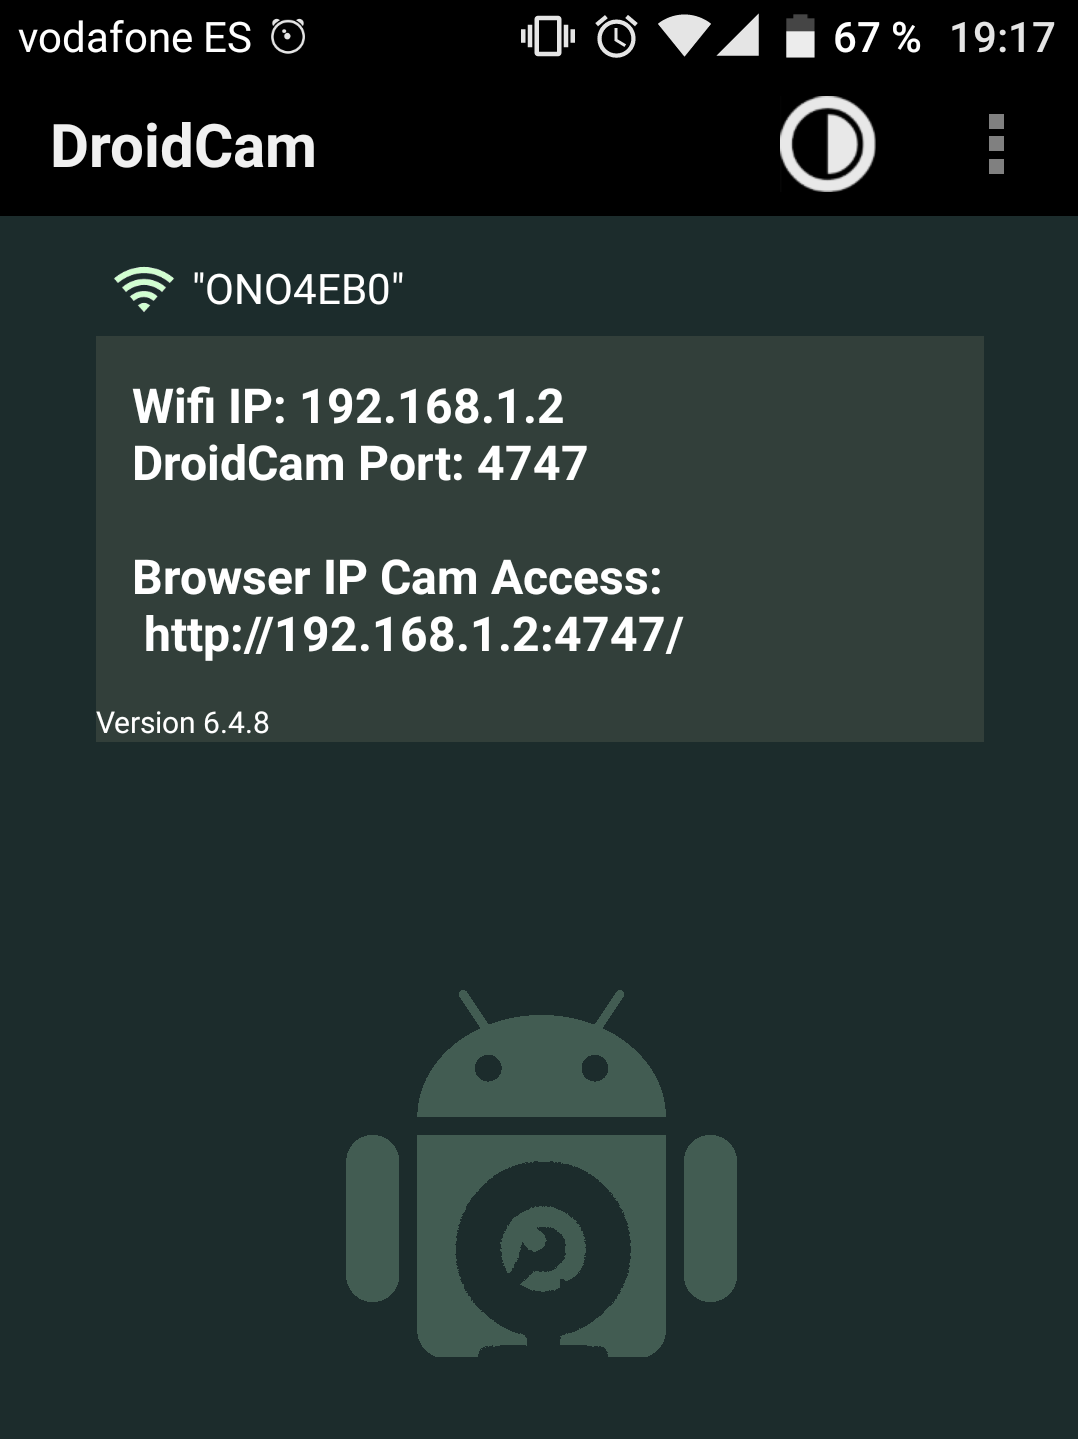
\includegraphics[width=0.9\linewidth]{figures/droidcampre.png}
		\caption{}
	\end{subfigure}%
	\begin{subfigure}{0.33\textwidth}
		\centering
		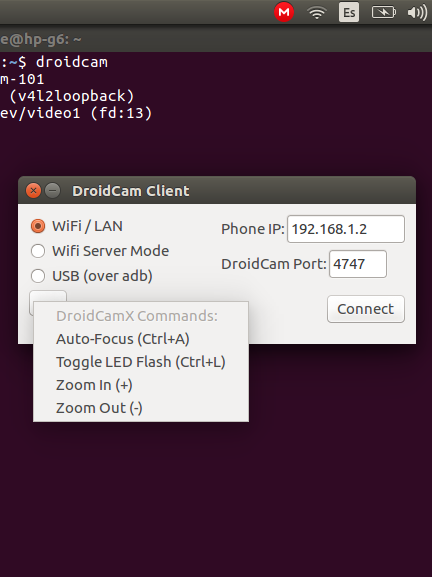
\includegraphics[width=0.9\linewidth]{figures/droidcamlinux.png}
		\caption{}
	\end{subfigure}%
	\begin{subfigure}{0.33\textwidth}
		\centering
		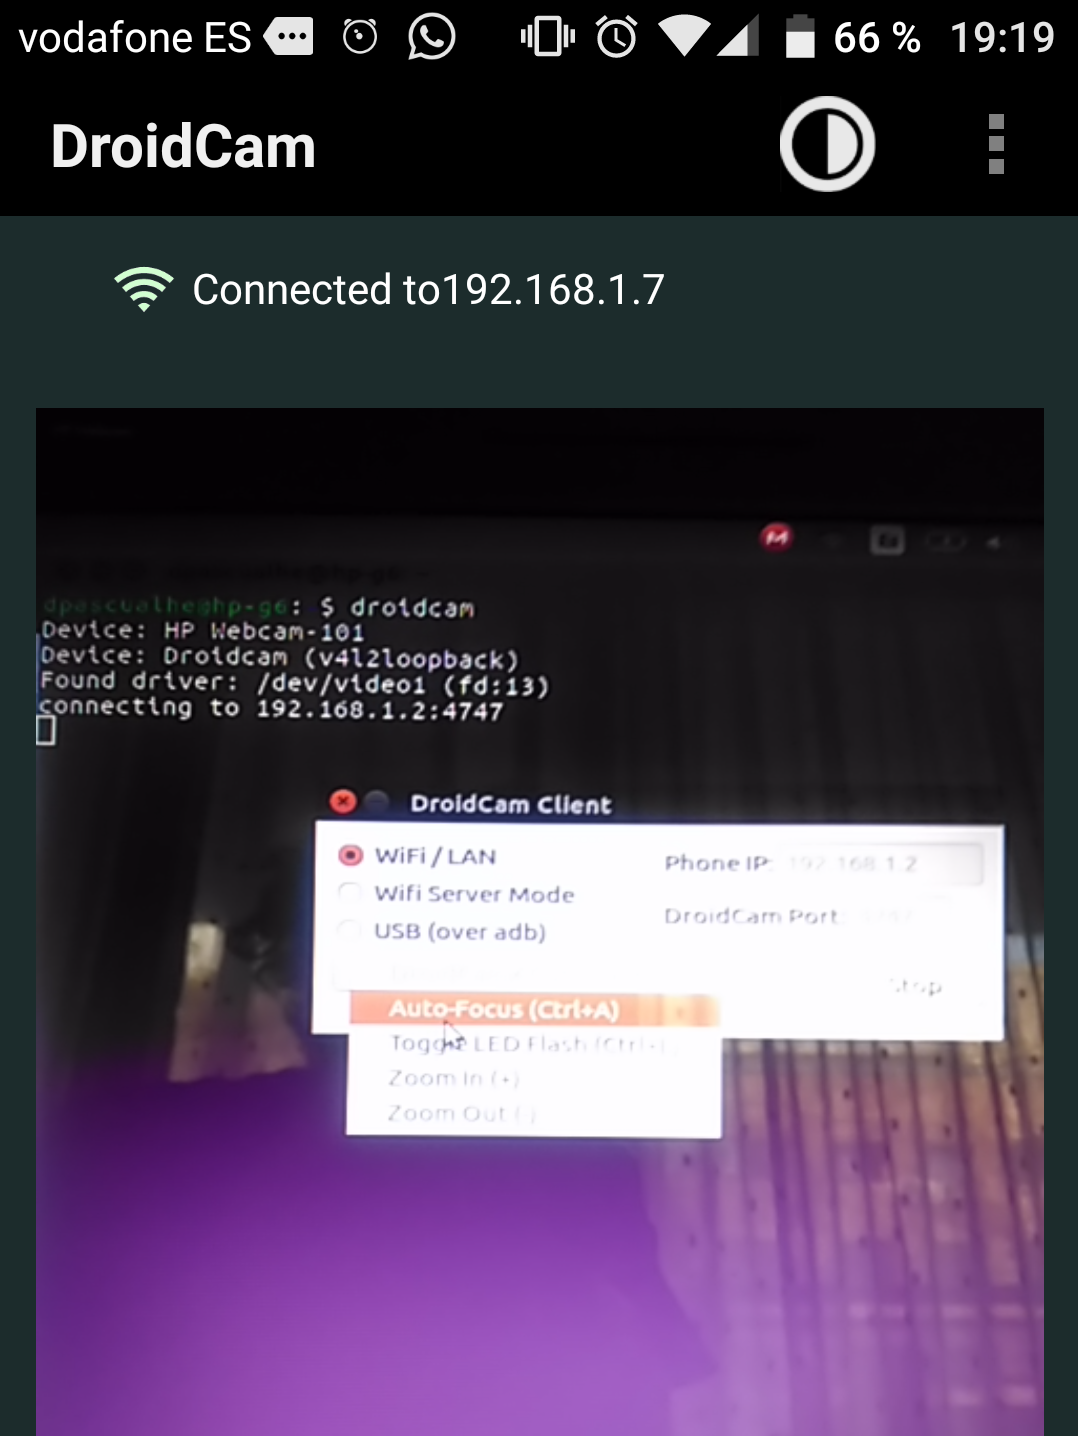
\includegraphics[width=0.9\linewidth]{figures/droidcampost.png}
		\caption{}
	\end{subfigure}
	\caption{Droidcam usage: (a) Android server; (b) Linux client; (c) connection established.}
	\label{fig:droidcam}
\end{figure}

JdeRobot \textit{cameraserver} driver cleanly connects to the camera device that the DroidCam Linux client provides in the host computer when attached to the DroidCam Android app.